% Created 2022-01-04 Tue 01:03
% Intended LaTeX compiler: pdflatex
\documentclass[presentation]{beamer}
\usepackage[utf8]{inputenc}
\usepackage[T1]{fontenc}
\usepackage{graphicx}
\usepackage{grffile}
\usepackage{longtable}
\usepackage{wrapfig}
\usepackage{rotating}
\usepackage[normalem]{ulem}
\usepackage{amsmath}
\usepackage{textcomp}
\usepackage{amssymb}
\usepackage{capt-of}
\usepackage{hyperref}
\usepackage{awesomebox}
\usepackage{booktabs}
\usepackage{placeins}
\usepackage{siunitx}
\usepackage{minted}
\usetheme[progressbar=frametitle]{metropolis}
\usepackage{tikz}
\usepackage{tikz-3dplot}
\usepackage{pgfplots}
\pgfplotsset{compat=newest}
\usepackage{spot}
\usetikzlibrary{calc,patterns,decorations.pathmorphing,decorations.markings}
\usepgfplotslibrary{groupplots}
\newcommand{\gv}[1]{\ensuremath{\mbox{\boldmath$ #1 $}}}
\newcommand{\bv}[1]{\ensuremath{\mathbf{#1}}}
\newcommand{\norm}[1]{\left\lVert#1\right\rVert}
\newcommand{\abs}[1]{\left\lvert#1\right\rvert}
\newcommand{\bigqm}[1][1]{\text{\larger[#1]{\text{?}}}}
\newcommand{\order}[1]{\mathcal O \left( #1 \right)} % order of magnitude
\definecolor{scarlet}{rgb}{1.0, 0.13, 0.0}
\definecolor{shamrockgreen}{rgb}{0.0, 0.62, 0.38}
\definecolor{royalblue}{rgb}{0.25, 0.41, 0.88}
\definecolor{metropolisorange}{RGB}{235,129,27}
\definecolor{metropolisblue}{RGB}{35,55,59}
\usetheme{default}
\author{\emph{Tejaswin Parthasarathy}, Mattia Gazzola}
\date{\today}
\title{Elastica : Timesteppers}
\subtitle{ME447: Comp. Design \& Dyn. of Soft Syst}
\hypersetup{
 pdfauthor={\emph{Tejaswin Parthasarathy}, Mattia Gazzola},
 pdftitle={Elastica : Timesteppers},
 pdfkeywords={},
 pdfsubject={},
 pdfcreator={Emacs 28.0.50 (Org mode 9.4.6)}, 
 pdflang={English}}
\begin{document}

\maketitle
\tikzset{>=latex}
\section{Time-marching algorithms}
\label{sec:org3fd3f69}
\begin{frame}[label={sec:orgc24348f}]{Motivation}
\begin{example}[Solve the following ODE]
\[ \frac{dx}{dt} = 2x \quad x(0) = 1 \]
\end{example}
\begin{block}{We can!}
\[ x(t) = e^{2t}\]
\end{block}
\end{frame}

\begin{frame}[label={sec:orgb6c16ac}]{Motivation}
\begin{example}[Solve the following ODE]
\[ \frac{dx}{dt} = \sin(\cos x^{\frac{4}{3}}) + 4\sin^2(t) \quad x(0) = 1 \]
\end{example}

\begin{block}<2->{We can!}
Use a time-marching algorithm that can solve the above equation, albeit numerically
\end{block}
\end{frame}
\begin{frame}[label={sec:org79f0b8c}]{Introduction}
\begin{itemize}
\item As seen in the last lecture, all our (temporal/spatial) rate of frame change
vectors (that effect rotations) are precisely of this form
\end{itemize}

More generally, we can solve problems of the form
\[ \frac{\partial \mathbf{u}}{\partial t} = \mathbf{F}(\mathbf{u}, t) \]
which is a partial differential equation (PDE), wherein \(\mathbf{F}\) is
any arbitrary function.
\end{frame}
\begin{frame}[label={sec:org38ebce7}]{Examples}
\begin{itemize}
\item Population dynamics (Lotka-Volterra)
\[ \begin{aligned}
	  y'_1 &= y_1 (\alpha_1 - \beta_1 y_2) \quad \text{(prey)} \\
	  y'_2 &= y_2 (-\alpha_2 + \beta_2 y_1) \quad \text{(predator)}
	  \end{aligned} \]
\item Chemical reactions (stiff)
\item Newton's equations of motion (our focus)
\[  m\ddot{\gv{x}} = F(\gv{x},t) \]
\end{itemize}
\note{:B\_note:
\begin{itemize}
\item Need not be time variable
\end{itemize}}
\end{frame}
\begin{frame}[label={sec:orgd98aec1}]{Introduction}
\begin{itemize}
\item We investigate three different (classes of) time-marching algorithms for
autonomous problems (?!):
\begin{itemize}
\item Euler's method (or Euler forward/backward)
\item Runge-Kutta-4/RK4 (multi-stage methods)
\item Position Verlet (symplectic, area preserving integrators)
\end{itemize}
\item We develop time marching methods that compute approximations to \(u(t)\)
at specfic time points, \(t^0, t^1, \cdots, t^n\).
\begin{itemize}
\item We only consider a uniform timestep size \(dt  \rightarrow t^n = n \cdot
       dt\).
\end{itemize}
\item Finally, we \emph{compare} these methods based on general and problem-specific properties\ldots{}
\end{itemize}
\end{frame}
\begin{frame}[label={sec:orgb10ecc6}]{Problem statement}
\begin{itemize}
\item Need function \(\gv{u} : [0, T] \to \mathbb{R}^n\) so that
\begin{itemize}
\item \(\gv{u}^{(k)}(t) = \gv{f}(t, \gv{u}, \gv{u}', \cdots , \gv{u}^{(k-1)})\) (\alert{explicit})
\end{itemize}
or
\begin{itemize}
\item \(\gv{f}(t, \gv{u}, \gv{u}', \cdots , \gv{u}^{(k-1)}, \gv{u}^{(k)}) = \gv{0}\) (\alert{implicit})
\end{itemize}
where we find a solution to a \(k\)-th order ordinary differential
equation. Typically \(k = 1,2\)
\item Meaningful only when accompanied by \(k\) initial conditions
\end{itemize}
\end{frame}
\begin{frame}[label={sec:orgfa4ae8a}]{Some properties of ODEs}
\begin{itemize}
\item \alert{Autonomous} ODE?
\begin{itemize}
\item \(\gv{f}\) does not explicitly depend on time \(t\)
\item An ODE can be made autonomous by introducing an extra variable (More on
this later)
\end{itemize}
\item \alert{Linear} ODE?
\begin{itemize}
\item \(\gv{f}(\gv{u}, t) =  \bv{A}(t)\gv{u} + \underbrace{\gv{b}}_{\text{forcing}}\)
\end{itemize}
\item \alert{Linear, homogenous} ODE?
\begin{itemize}
\item \(\gv{f}(\gv{u}, t) =  \bv{A}(t)\gv{u}\)
\end{itemize}
\item \alert{Constant-coefficient} ODE?
\begin{itemize}
\item \(\gv{f}(\gv{u}, t) =  \bv{A}\gv{u}\)
\end{itemize}
\end{itemize}
\end{frame}
\begin{frame}[label={sec:org2600374}]{Numerical methods: Euler's forward method}
\begin{columns}
\begin{column}{0.5\columnwidth}
\begin{itemize}
\item Simplest timestepping scheme
\item First-order approximation at time \(t_0\)
\begin{itemize}
\item Geometrical description
\item Taylor series expansion
\end{itemize}
\end{itemize}
\end{column}
\begin{column}{0.4\columnwidth}
\begin{center}
	\begin{tikzpicture}[
	declare function={func(\x)=sin(deg(pi*\x));},
	declare function={funcder(\x)=pi*cos(deg(pi*\x));}]
	\begin{axis}%
		[grid=none,
		axis x line=bottom,
		axis y line=left,
		domain=0.41:0.57,
		xmin=0.38,
		xmax=0.6,
		ymin=0.95,
		ymax=1.01,
		xlabel={$t$},
		ylabel={$u(t)$},
		ticks=none,
		height=1.12\textwidth,
		enlargelimits=false,
		]
		\addplot[smooth, very thick,
		color=metropolisorange]{func(x)};
		% For each in pgfplots is painful, see
		% https://tex.stackexchange.com/q/264168
		\addplot[thick, color=metropolisblue, mark=*] coordinates
		{ (0.41, {func(0.41)}) ({0.45}, {func(0.41) + funcder(0.41)*0.04}) };
		\foreach \a in {0.45, 0.49,..., 0.57}
        {\edef
		\temp{
		% \noexpand\addplot coordinates { (\x,0.96) (\x,1.02)};
		\noexpand\addplot[thick, color=metropolisblue, mark=*] coordinates
		{ (\a, {func(\a - 0.04) + funcder(\a - 0.04)*0.04}) ({\a + 0.04}, {func(\a) + funcder(\a)*0.04}) };
		}\temp
		}

		%\pgfplotsinvokeforeach {0.41, 0.45,..., 0.53}{
		% \addplot{\a*x^2};
		% \addplot coordinates { (#1, {func(#1)}) ({#1 + 0.04}, {func(#1) + funcder(#1)*0.04}) };
		% \addplot coordinates { (#1, #1) (#1 + 0.04, #1 + 0.04) };
		% \draw (axis cs:#1, func(#1)) -- (axis cs:{#1 + 0.04}, {func(#1) + funcder(#1)*0.04});
		% }
	\end{axis}
	\end{tikzpicture}
\end{center}
\end{column}
\end{columns}
\[ u(t_{0}+dt)=u(t_{0})+dt \cdot u'(t_{0})+{\frac {1}{2}}dt^{2} \cdot u''(t_{0})+O(dt^{3}). \]
\begin{itemize}
\item First order because local slope approximation is \(\order{dt}\)
\end{itemize}
\end{frame}

\begin{frame}[label={sec:org3b4075b}]{General explicit time stepping schemes}
\begin{itemize}
\item Explicit schemes approximate the next iterate \(t^{n+1}\) using:
\end{itemize}
\[ \gv{u}^{n+1} = \sum_{i=0}^{k} \alpha_i \gv{u}^{n-i} + \sum_{j=0}^{r} \beta_j \frac{\partial \gv{u}^{n-j}}{\partial t} \]
  which for \(k=1\) and \(r=0\) looks something along these lines:
\[ \gv{u}^{n+1} = \alpha_0 \gv{u}^{n} + \alpha_1 \gv{u}^{n-1} + \beta_0 \frac{\partial \gv{u}^{n}}{\partial t} \]
\begin{itemize}
\item Derivation of schemes other than Euler method follow a similar line of reasoning, while
details vary\footnote{By a \alert{lot}}
\end{itemize}
\end{frame}
\begin{frame}[label={sec:org4bc84f4}]{Some more time stepping schemes}
With \(\dot{x} = f(x)\),
\begin{block}{Euler forward}
\[ x^{n+1} = x^{n} + f(x^{n}) \cdot dt \]
\end{block}
\begin{block}{Euler backward}
\[ x^{n+1} = x^{n} + f(x^{n+1}) \cdot dt \]
\end{block}
\begin{columns}
\begin{column}{0.5\columnwidth}
\begin{block}{Midpoint method}
\begin{equation*}
\begin{aligned}
x^{*}&= x^{n} + f({x}^{n}) \cdot \frac{dt}{2} \\
x^{n+1} &= x^{n} + f({x}^{*}) \cdot dt \\
\end{aligned}
\end{equation*}
\end{block}
\end{column}
\begin{column}{0.4\columnwidth}
\begin{center}
	\begin{tikzpicture}[
	declare function={func(\x)=sin(deg(pi*\x));},
	declare function={funcder(\x)=pi*cos(deg(pi*\x));}]
	\begin{axis}%
		[grid=none,
		axis x line=bottom,
		axis y line=none,
		domain=0.43:0.49,
		xmin=0.41,
		xmax=0.51,
		ymin=0.975,
		ymax=1.005,
		ticks=none,
		height=1.1\textwidth,
		enlargelimits=false,
		clip=false]
		\addplot[smooth, very thick,
		color=metropolisorange]{func(x)} node[pos=0.1, above, anchor=south east]
		{{\scriptsize$x(t)$}};

		% Draw derivatve from yn to yn+1 first
		% 0.44 to 0.48
		\addplot[color=metropolisblue, mark=*] coordinates
		{ (0.44, {func(0.44)}) ({0.48},
		{func(0.44) + 0.04*funcder(0.46)-0.004}) }
		node[pos=0, below right, anchor=west]{{\scriptsize $y^n$}}
		node[below right, anchor=north west]{{\scriptsize $y^{n+1}$}}
		node[right, anchor=south west]{Estd.};

		% Draw actual derivatve line
		\addplot[color=royalblue, thick] coordinates
		{ (0.44, {func(0.46) - 0.02*funcder(0.46) }) (0.48,
		{func(0.46) + 0.02*funcder(0.46)}) } node[above]{Actual};

		% Draw connections to ground now
		\addplot[dashed] coordinates
		{ (0.44, {func(0.44)}) (0.44,\pgfkeysvalueof{/pgfplots/ymin})}
		node [above right, anchor=south west]{{\scriptsize$t^{n}$}};

		\addplot[dashed] coordinates
		{ (0.46, {func(0.46)}) (0.46,\pgfkeysvalueof{/pgfplots/ymin})}
		node [below, anchor=north]{{\scriptsize$t^{n} + \frac{dt}{2}$}};

		\addplot[dashed] coordinates
		{ (0.48, {func(0.48)}) (0.48,\pgfkeysvalueof{/pgfplots/ymin})}
		node [above right, anchor=south west]{{\scriptsize$t^{n+1}$}};

	\end{axis}
	\end{tikzpicture}
\end{center}
\end{column}
\end{columns}
\end{frame}
\begin{frame}[label={sec:org3bf8753}]{Some more time stepping schemes}
\begin{block}{Runge Kutta-4}
\begin{equation*}
\begin{aligned}
{k}_1 &= {f}({x}^{n}) \cdot dt \\
{k}_2 &= {f}({x}^{n} + 0.5 \cdot {k}_1)\cdot dt \\
{k}_3 &= {f}({x}^{n} + 0.5 \cdot {k}_2)\cdot dt \\
{k}_4 &= {f}({x}^{n} + {k}_3)\cdot dt \\
{x}^{n+1} &= {x}^{n} + \frac{{k}_1+2{k}_2+2{k}_3+{k}_4}{6}
\end{aligned}
\end{equation*}
\end{block}
\begin{block}{Position/Velocity Verlet}
\begin{itemize}
\item Later on we introduce these two schemes in the context of integrating
second order ODEs
\end{itemize}
\end{block}
\end{frame}
\begin{frame}[label={sec:orgb1d9e79}]{Function evaluations}
\begin{itemize}
\item Our first attempt at comparing schemes is the number of functional
evaluations for one time step\ldots{}
\item Why? \(f(x)\) can be expensive to evaluate (e.g. calculating the effect
of the energy diffusion on millions to billions of
grid points in an astrophysical simulation)
\end{itemize}
\begin{table}[htbp]
\caption{\label{tab_sym_snake_params}Number of function evaluations for schemes}
\centering
\begin{tabular}{lr}
\toprule
Scheme & \(n[f(x)]\)\\
\midrule
Euler fwd & 1\\
Euler bwd & Solve!\\
Midpoint & 2\\
RK4 & 4\\
Verlet* & 1\\
\bottomrule
\end{tabular}
\end{table}
\end{frame}
\begin{frame}[label={sec:orge2303a5}]{Convergence/ Consistency}
Suppose the numerical solution at some time \(t\) is \(\gv{u}\), and the
exact solution at the same time is \(\tilde{\gv{u}}\).
\begin{definition}[Convergence]
A numerical method is said to be convergent if the numerical solution
approaches the exact solution as the step size \(dt\) goes to 0.
\end{definition}
The methods we just looked at are all convergent.
\begin{definition}[Consistency]
A numerical method is said to be consistent if the error, \(e_{dt}:=\lVert\tilde{\gv{u}}-\gv{u} \rVert\) is such that
\[ \lim_{dt \to 0} \frac{e_{dt}}{dt} = 0\]
\end{definition}
\end{frame}
\begin{frame}[label={sec:org2500b2a}]{Order of convergence}
\begin{definition}[Order of accuracy]
The numerical solution \(\gv{u}\) is said to be \(p^{\text{th}}\)-order
accurate if the error, \(e(dt):=\lVert\tilde{\gv{u}}-\gv{u} \rVert\)
is proportional to the step-size \(dt\), to the \(p^{\text{th}}\) power. That
is
\[ e(dt)=\lVert\tilde{\gv{u}}-\gv{u} \rVert\leq C(dt)^{p} \]
where the constant \(C\) is independent of \(dt\) and usually depends on
the solution \(\gv{u}\)
\end{definition}
 In the big O notation an \(p^{\text{th}}\)-order accurate numerical method
 is notated as
\[ \lVert\tilde{\gv{u}}-\gv{u} \rVert = \order{h^p}\]
\end{frame}
\begin{frame}[label={sec:org984fd76}]{Order of convergence : Importance}
\begin{columns}
\begin{column}{0.32\columnwidth}
\begin{block}{First order}
\begin{center}
\begin{tabular}{ll}
\toprule
\(dt\) & \(e(dt)\)\\
\midrule
\(10^{-1}\) & \(1\)\\
\(10^{-2}\) & \(10^{-1}\)\\
\(10^{-3}\) & \(10^{-2}\)\\
\(10^{-4}\) & \(10^{-3}\)\\
\(10^{-5}\) & \(\spot<2>{10^{-4}}\)\\
\bottomrule
\end{tabular}
\end{center}
\end{block}
\end{column}

\begin{column}{0.32\columnwidth}
\begin{block}{Second order}
\begin{center}
\begin{tabular}{ll}
\toprule
\(dt\) & \(e(dt)\)\\
\midrule
\(10^{-1}\) & \(1\)\\
\(10^{-2}\) & \(10^{-2}\)\\
\(10^{-3}\) & \(10^{-4}\)\\
\(10^{-4}\) & \(10^{-6}\)\\
\(10^{-5}\) & \(\spot<2>{10^{-8}}\)\\
\bottomrule
\end{tabular}
\end{center}
\end{block}
\end{column}
\begin{column}{0.32\columnwidth}
\begin{block}{Fourth order}
\begin{center}
\begin{tabular}{ll}
\toprule
\(dt\) & \(e(dt)\)\\
\midrule
\(10^{-1}\) & \(1\)\\
\(10^{-2}\) & \(10^{-4}\)\\
\(10^{-3}\) & \(10^{-8}\)\\
\(10^{-4}\) & \(10^{-12}\)\\
\(10^{-5}\) & \(\spot<2>{10^{-16}}\)\\
\bottomrule
\end{tabular}
\end{center}
\end{block}
\end{column}
\end{columns}
\begin{alertblock}<2->{Better returns for same timestep!}
\end{alertblock}
\end{frame}

\begin{frame}[label={sec:org9ae791f}]{Order of convergence : Implementation}
\begin{block}{Model problem definition}
Let's solve this problem, and test out methods for convergence:
\[ \frac{dy}{dt} = -y \quad,\quad  y(0) = 1 \]
which as we know has the analytical solution \(\tilde{y}(t) = e^{-t}\) \(\rightarrow\)
error known at every \(dt\)

Notice:
\begin{itemize}
\item We choose a simple problem to understand performance/convergence
\begin{itemize}
\item More complicated problems usually follow suit
\end{itemize}
\item We are solving an eigenvalue problem, just like the last lecture (rotations)
\end{itemize}

\alert{ACTIVITY}
\end{block}
\end{frame}
\begin{frame}[label={sec:org2bd73fe}]{Order of accuracy : Results}
% Need to run the notebook first
\begin{center}
	\begin{tikzpicture}
		\begin{loglogaxis}[
			enlargelimits=true,
			grid=both,
			grid style={line width=.1, draw=gray!20},
			major grid style={line width=.2,draw=gray!50},
			xlabel=$dt$,
			ylabel=$e(dt)$,
			height=1.0\textheight
			]
			% Euler backward/forward
			\addplot [mark=*, mark size=2.5, scarlet, very thick]
			table {code/data/euler_bwd_ooa.txt} node [midway, above left, anchor=south east]
			{Euler bwd/fwd};
			\addplot [metropolisblue, dashed, thick]
			table {code/data/euler_bwd_ooa_slopes.txt};

			% Midpoitn
			\addplot [mark=*, mark size=2.5, royalblue, very thick]
			table {code/data/midpoint_method_ooa.txt} node [pos=0.8, below , anchor=north west]
			{Midpoint};
			\addplot [metropolisblue, dashed, thick]
			table {code/data/midpoint_method_ooa_slopes.txt};

			% RK4
			\addplot [mark=*, mark size=2.5, metropolisorange, very thick]
			table {code/data/rk4_ooa.txt} node [midway, below right, anchor=north west]
			{RK4};
			\addplot [metropolisblue, dashed, thick]
			table {code/data/rk4_ooa_slopes.txt};

		\end{loglogaxis}
	\end{tikzpicture}
\end{center}
\end{frame}

\begin{frame}[label={sec:orga06aaa8}]{Order of accuracy : Results}
\begin{table}[htbp]
\caption{\label{tab_sym_snake_params}Order of accuracy for different schemes}
\centering
\begin{tabular}{lr}
\toprule
Scheme & \(p\)\\
\midrule
Euler & 1\\
Midpoint & 2\\
RK4 & 4\\
Verlet* & ?\\
\bottomrule
\end{tabular}
\end{table}
\end{frame}
\begin{frame}[label={sec:org70a597c}]{Bottomline}
\begin{itemize}
\item Order of accuracy is a measure of ``goodness'' of algorithm
\item Higher-order accurate algorithms commit less error for a given \(h\).
\item But they are costly (in terms number of function evaluations, and
ultimately number of operations performed)
\end{itemize}
\end{frame}
\begin{frame}[label={sec:org492de25}]{Higher order ODEs}
We consider a harmonic oscillator, i.e. a linear spring-mass system:
\[ \ddot{x} + \omega^2 x = 0\]
\begin{columns}
\begin{column}{0.6\columnwidth}
\begin{itemize}
\item \(\omega^2 = \frac{k}{m} \equiv 1\)
\item Consider \(x(0) = 1, \dot{x}(0) = 0\) (need two ICs)
\item Solution is analytically known to be
\end{itemize}
\[ x(t) = \cos(t) \quad \dot{x}(t) = -\sin(t) \]
\begin{itemize}
\item Notice : solution is bounded
\end{itemize}
\end{column}
\begin{column}{0.4\columnwidth}
\tikzset{boxstyle/.style={draw,outer sep=0pt,thick}}
% https://tex.stackexchange.com/a/13952
\begin{center}
	\begin{tikzpicture}[scale=1]
	\tikzstyle{spring}=[thick,decorate,color=metropolisblue, decoration={zigzag,pre length=4,post length=4,segment length=10}]
	\tikzstyle{ground}=[fill,pattern=north east lines,draw=none,minimum width=8,minimum height=3]

	\node (M) [boxstyle, minimum width=50, minimum height=50, color=metropolisblue] {$m$};

	\node (ground) [ground,anchor=north,yshift=-10,minimum width=80] at (M.south) {};
	\draw (ground.north east) -- (ground.north west);
	\draw [thick] (M.south west) ++ (8pt,-5pt) circle (5pt) (M.south east) ++ (-8pt,-5pt) circle(5pt);
	% \draw [thick] (M.south west) ++ (8,-5) circle[radius=5pt];
	% \draw [thick]

	\node (wall) [ground, rotate=-90, minimum width=80, xshift=-10, yshift=-80] {};
	\draw (wall.north east) -- (wall.north west);

	% Syntax ($(A)!(C)!(B)$), specifies the projection of (C) on the line
	% from (A) to (B),
	% <name>.<number> syntax https://tex.stackexchange.com/a/426804
	\draw [spring] (M.180) -- ($(wall.north east)!(M.180)!(wall.north west)$)
	node [midway, above]{$kx$};

	% Draw x position beginning and end
	% Interesection of north east ground with horizontal wall and 10 pt line
	\draw [thick, color=metropolisblue] ($(wall.south west)!(ground.north west)!(wall.north west)$) --
	++ (0pt,-5pt) coordinate (c) -- ++(0pt,-5pt);
	\draw [thick, color=metropolisblue, ->] (c) -- ($(M.south west)!(c)!(M.north west)$)
	node[right]{$x$};

	\end{tikzpicture}
\end{center}
\end{column}
\end{columns}
\end{frame}

\begin{frame}[label={sec:org5b1d4e0}]{Conservation laws in typical higher order ODEs}
The system is \alert{Hamiltonian} as the energy is conserved:
\[ \underbrace{H(x(t), \dot{x}(t))}_{\text{Hamiltonian/total energy}} = \underbrace{x^2(t)}_{\text{Potential energy}} +
   \underbrace{\dot{x}^2(t)}_{\text{Kinetic energy}} \equiv 1\]

The solution can be represented in the time domain (left) or in the phase
portrait (right)
\begin{columns}
\begin{column}{0.5\columnwidth}
\begin{center}
	\begin{tikzpicture}
	\begin{axis}%
		[grid=both,
		minor tick num=4,
		grid style={line width=.1pt, draw=gray!10},
		major grid style={line width=.2pt,draw=gray!50},
		axis lines=middle,
		domain=0:7,
		x label style={at={(axis description cs:1.1,0.5)},anchor=east},
		y label style={at={(axis description cs:-0.1,.5)},rotate=90,anchor=south},
		xlabel={$t$},
		ylabel={$u(t)$},
		width=1.1\textwidth,
		title style={at={(0.5,0)},anchor=north,yshift=-0.1},
		title={Time domain},
		enlargelimits=true,
		% enlargelimits={abs=0.2}
		]
		\addplot[samples=200,smooth,metropolisorange,very thick]{cos(deg(x))}
		node[pos=0.1, right]{{\small $x(t)$}};
		\addplot[samples=200,smooth,metropolisblue,very thick]{-sin(deg(x))}
		node[pos=0.99, below left, anchor=north east]{{\small $\dot{x}(t)$}};
	\end{axis}
	\end{tikzpicture}
\end{center}
\end{column}
\begin{column}{0.5\columnwidth}
\begin{center}
	\begin{tikzpicture}
	\begin{axis}%
		[grid=both,
		minor tick num=4,
		grid style={line width=.1pt, draw=gray!10},
		major grid style={line width=.2pt,draw=gray!50},
		axis lines=middle,
		width=1.1\textwidth,
		xmin=-1.1, xmax=1.1, ymin=-1.1, ymax=1.1,
		axis equal,
		x label style={at={(axis description cs:0.98,0.5)},anchor=south east},
		y label style={at={(axis description cs:0.5,0.98)},anchor=west},
		xlabel={\textcolor{metropolisorange}{$x$}},
		ylabel={\textcolor{metropolisblue}{$\dot{x}$}},
		title style={at={(0.5,-0.2)},anchor=south},
		% title style={at={(0.5,0.0)},anchor=north},
		title={Phase portrait},
		enlargelimits=true,
		disabledatascaling
		]
		\draw[very thick, black] (axis cs: 0, 0) circle [radius=1];
		\draw[thick, black, ->] (axis cs:0, 0)--(axis cs:0.707106, 0.707106);
		\draw [thick,->] (0.4,0) arc (0:45:0.4) node [midway, right]{{\scriptsize $t$}};
	\end{axis}
	\end{tikzpicture}
\end{center}
\end{column}
\end{columns}
\end{frame}

\begin{frame}[label={sec:org8359662}]{Conversion to lower order ODE}
Let's convert the second order ODE to two first order ODEs, by considering \(y = \dot{x} \Rightarrow\)
\[ \begin{pmatrix} \dot{x} \\ \dot{y} \end{pmatrix} = \begin{bmatrix} 0 & 1\\-1
   & 0 \end{bmatrix} \begin{pmatrix} {x} \\ {y} \end{pmatrix} \]

\begin{itemize}
\item You can reuse the same schemes!
\item Alternatively, we can develop schemes for the second order equation
directly : \alert{Example using Taylor series}
\end{itemize}

\begin{block}{Position Verlet scheme}
\begin{itemize}
\item For integrating equations similar to \(\ddot{\gv{x}} = \gv{f}(\gv{x})\),
with \(\gv{y} = \dot{\gv{x}}\)
\end{itemize}
\begin{equation*}
\begin{aligned}
\gv{x}^* &= \gv{x}^n + 0.5\cdot dt \cdot \gv{y}^n \\
\gv{y}^{n+1} &= \gv{y}^n + dt \cdot \gv{f}\left( \gv{x}^*\right) \\
\gv{x}^{n+1} &= \gv{x}^* + 0.5\cdot dt \cdot \gv{y}^{n+1}
\end{aligned}
\end{equation*}
\end{block}
\note{:B\_note:
\begin{itemize}
\item Show derivation using
\end{itemize}
\[ f(x+h) = f(x) + f'(x)h + f''(x)h^2/2! + \cdots \quad
	f(x - h) = f(x) - f'(x) h + f''(x)h^2/2! + \cdots \]
and add them up}
\end{frame}
\begin{frame}[label={sec:org61a1641}]{More schemes}
Another example of a scheme for this model equation is
\begin{block}{Velocity Verlet algorithm}
\begin{equation*}
\begin{aligned}
\gv{y}^* &= \gv{y}^n + 0.5\cdot dt \cdot \gv{f}\left( \gv{x}^n\right) \\
\gv{x}^{n+1} &= \gv{x}^{n} + dt \cdot \gv{y}^{*} \\
\gv{y}^{n+1} &= \gv{y}^* + 0.5\cdot dt \cdot \gv{f}\left( \gv{x}^{n+1}\right) \\
\end{aligned}
\end{equation*}
\end{block}
\begin{block}{How do these schemes fare?}
\begin{itemize}
\item Position and Velocity Verlet have \(p = 2\) (second-order accurate) for
both position \(\gv{x}\) and velocity \(\gv{y}\)
\item But Position Verlet has only \alert{one} function evaluation!
\end{itemize}
\end{block}
\end{frame}
\begin{frame}[label={sec:org4f35c6d}]{Energy-preserving/symplectic schemes}
\begin{block}{Why do we even care about these schemes?}
\begin{itemize}
\item Clearly, RK4 has higher order of convergence and it must be better?
\end{itemize}
\end{block}
\begin{block}{Answer}
\begin{itemize}
\item Position and Velocity Verlet schemes are symplectic (area-preserving) schemes
\item They preserve in the phase-portrait of a Hamiltonian system \(\Rightarrow\)
They always conserve energy by design!
\end{itemize}

\alert{ACTIVITY}
\end{block}
\end{frame}
\begin{frame}[label={sec:orga5817e9}]{Energy-preserving/symplectic schemes}
\begin{itemize}
\item The harmonic equation arises from Newton's fundamental laws of motion,
without dissipative forces \(\Rightarrow\) energy needs to be conserved
\item RK4 slowly dissipates energy \(\Rightarrow\) unphysical!
\item Euler forward increases energy without bounds, even when physics dictates
bounded solutions (counter examples?)
\item Verlet schemes conserve energy even for large \(dt\)
\begin{itemize}
\item There are still errors (it still has \(p = 2\) ) in the \emph{phase}
\item \alert{DEMO}
\end{itemize}
\end{itemize}
\end{frame}
\begin{frame}[label={sec:org0a9e1a4}]{But why is it energy preserving?\footnote{Peter Young, \href{https://young.physics.ucsc.edu/242/leapfrog.pdf}{Course Notes:Physics 115/242}}}
\begin{itemize}
\item Because it preserves the area in the \(x-p\) phase space (thus the area-preserving
property seen earlier)
\item Why area preservation? \(\Rightarrow\) \alert{Liouville's theorem}
\item On one application of the time-stepping scheme (map), an initial rectangle
with side lengths \(dx , dp\) gets stretched to a parallelogram with
sides \(dx^\prime, dp^\prime\)
\end{itemize}

\begin{columns}
\begin{column}{0.6\columnwidth}
New area \(dA^\prime = \det \bv{J} dA\), where \(\bv{J}\) is
\[ \bv{J} =	\begin{bmatrix}
	\frac{\partial x^\prime}{\partial x} & \frac{\partial x^\prime}{\partial p}  \\
	\frac{\partial p^\prime}{\partial x} & \frac{\partial p^\prime}{\partial p}  \\
	\end{bmatrix} \]

In the case of symplectic schemes, we require \(\det \bv{J} = 1\)
\end{column}
\begin{column}{0.4\columnwidth}
\begin{figure}[htbp]
\centering
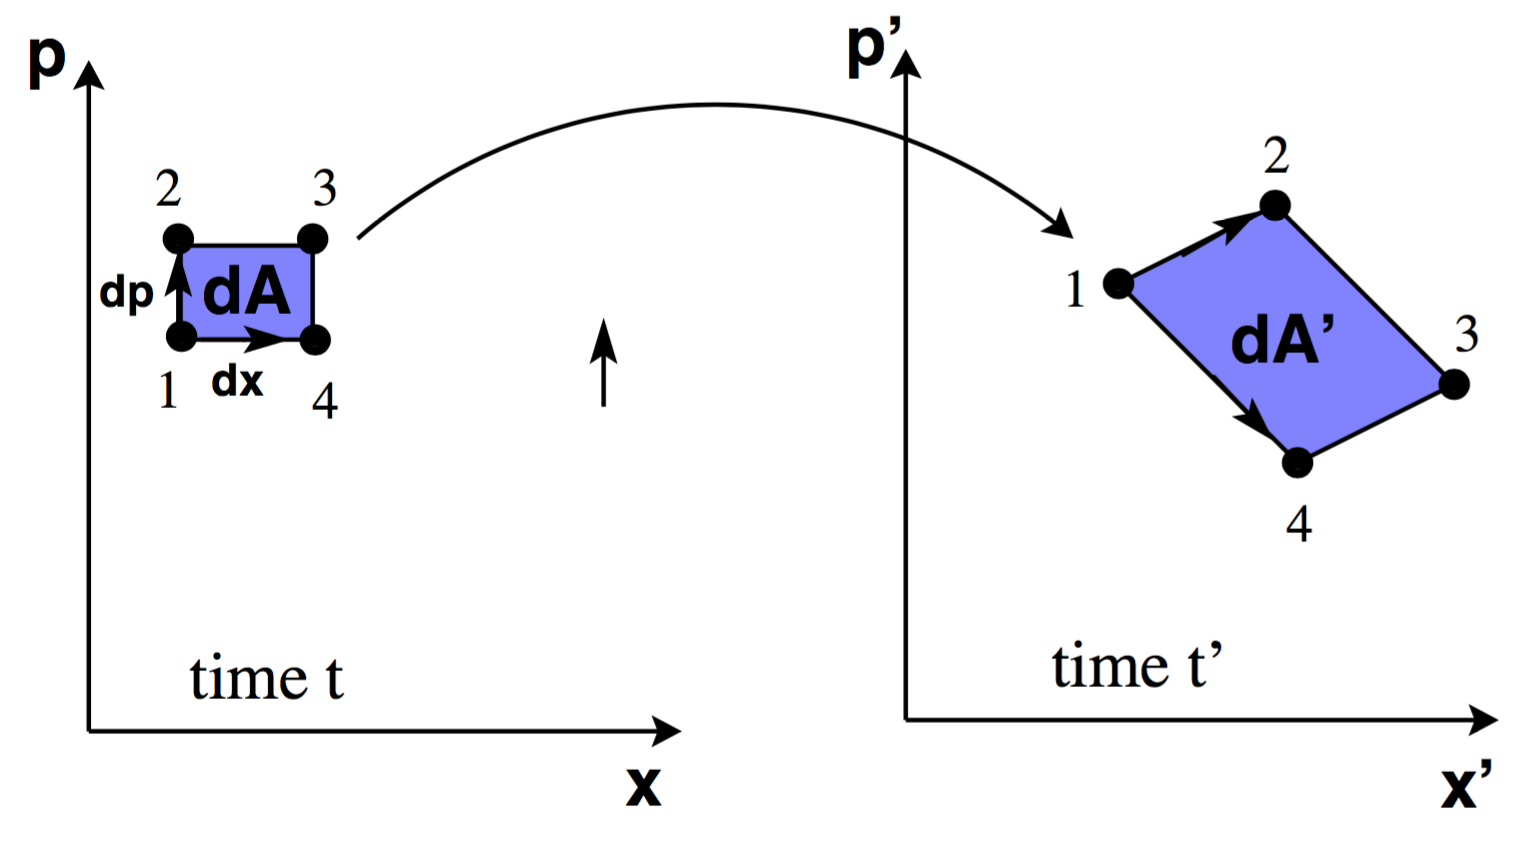
\includegraphics[width=1.0\textwidth]{images/area_preserve.png}
\caption{Area preservation}
\end{figure}
\end{column}
\end{columns}
\end{frame}
\begin{frame}[label={sec:org18a66f7}]{Area preserviation of Verlet and Euler algorithms}
From a different perspective,
\(\begin{pmatrix} \delta x_1 \\ \delta v_1 \end{pmatrix} = \bv{J}\begin{pmatrix} \delta x_0
   \\ \delta v_0 \end{pmatrix}\)
where subscripts denote number of applications of the time-stepping scheme.
Break it down to
\(\bv{J} = \bv{C}\bv{B}\bv{A}\).
\begin{columns}
\begin{column}{0.5\columnwidth}
\begin{alertblock}{Euler forward}
\begin{equation*}
\begin{aligned}
\bv{A} &= \begin{bmatrix} 1 & h\\ hF^\prime(x_0) & 1 \end{bmatrix}\\
\bv{B} &= \begin{bmatrix} 1 & 0\\ 0 & 1 \end{bmatrix} \\
\bv{C} &= \begin{bmatrix} 1 & 0\\ 0 & 1 \end{bmatrix}
\end{aligned}
\end{equation*}
\end{alertblock}
\end{column}
\begin{column}{0.5\columnwidth}
\begin{alertblock}{Position verlet}
\begin{equation*}
\begin{aligned}
\bv{A} &= \begin{bmatrix} 1 & \tfrac{h}{2}\\ 0 & 1 \end{bmatrix}\\
\bv{B} &= \begin{bmatrix} 1 & 0 \\ hF^\prime(x_{1/2}) & 1 \end{bmatrix}\\
\bv{C} &= \begin{bmatrix} 1 & \tfrac{h}{2}\\ 0 & 1 \end{bmatrix}\\
\end{aligned}
\end{equation*}
\end{alertblock}
\end{column}
\end{columns}
Calculate \(\det \bv{J}\)\ldots{}
\end{frame}
\begin{frame}[label={sec:orga4bc767}]{Bottomline}
\begin{itemize}
\item The evolution of dynamics of the soft filament also relies on some form of energy
conservation (translational/rotational/bending/twist/shear/stretch) as the
governing equations are Newton's laws
\item We need symplectic algorithms for maintaining relevance to the physical world
\end{itemize}

\alert{Counterpoint} In reality, there is always dissipation (frictional forces,
 viscous forces, drag forces not included in either of the above, etc.)
\end{frame}
\begin{frame}[label={sec:org907601a}]{Why did forward Euler blow-up?}
\begin{itemize}
\item Because it was unstable\ldots{}related to the stability of a method (alternatively instability)
\end{itemize}
\begin{block}{Euler forward algorithm}
\begin{itemize}
\item Find out what happens to the numerical solution using forward Euler when applied to
\(\dot{y}(t) = \lambda y(t)\)
\item Why? Eigenvalue problem, easy to extend analysis to general matrices
\end{itemize}
\begin{equation*}
\begin{aligned} y_k & = y_{k-1} + h \lambda y_{k-1} \\ &= (1 + h
\lambda)y_{k-1} \\ &= (1 + h \lambda)^{k}y_{0}
\end{aligned}
\end{equation*}
\begin{itemize}
\item So stability \(\Leftrightarrow\) \(\abs{1 + h \lambda} \leq 1\)
\end{itemize}
\end{block}
\end{frame}
\begin{frame}[label={sec:org91666ec}]{Why did forward Euler blow-up?}
\begin{itemize}
\item \(\abs{1 + h \lambda}\) is the \alert{amplification factor}
\item The condition on the amplification factor implies the existence of a
\alert{stability region} in the complex plane
\item \alert{DEMO}
\end{itemize}
% This file was created by matplotlib2tikz v0.7.4.
\begin{center}
\begin{tikzpicture}[scale=0.45]
	\begin{groupplot}[group style={group size=3 by 1}]
	\nextgroupplot[
	title={Euler forward},
	grid=both,
	grid style={line width=.1pt, draw=gray!10},
	major grid style={line width=.2pt,draw=gray!50},
	axis equal,
	xmin=-2.2, xmax=0.2,
	ymin=-1.2, ymax=1.2,
	minor tick num=4,
	xlabel={\(\displaystyle \mathrm{Re}\)},
	ylabel={\(\displaystyle \mathrm{Im}\)},
	enlargelimits=false,
	disabledatascaling
	]

	\draw[very thick, metropolisblue, fill=metropolisorange, fill opacity=0.3]
	(axis cs: -1, 0) circle [radius=1];
	% \addplot [very thick, metropolisorange, fill=metropolisorange, fill opacity=0.3]
	% table {code/data/euler_fwd_stability.txt};

	\nextgroupplot[
	title={Euler backward},
	grid=both,
	grid style={line width=.1pt, draw=gray!10},
	major grid style={line width=.2pt,draw=gray!50},
	axis equal,
	xmin=-0.2, xmax=2.2,
	ymin=-1.2, ymax=1.2,
	minor tick num=4,
	xlabel={\(\mathrm{Re}\)},
	enlargelimits=false,
	disabledatascaling
	]
	% \addplot [fill=metropolisorange, fill opacity=0.3]
	% table [row sep=\\]{
	% -0.5 -1.5\\
	% 2.5 -1.5\\
	% 2.5 1.5\\
	% -0.5 1.5\\
	% -0.5 -1.5};
	\filldraw[fill=metropolisorange, fill opacity=0.3]
	(axis cs: -1, -2) rectangle (3,2);
	\draw[very thick, metropolisblue, fill=white, fill opacity=0.6]
	(axis cs: 1, 0) circle [radius=1];
	% \addplot [thick, metropolisorange] table {code/data/euler_bwd_stability.txt};

	\nextgroupplot[
	title={Runge-Kutta--4},
	grid=both,
	grid style={line width=.1pt, draw=gray!10},
	major grid style={line width=.2pt,draw=gray!50},
	axis equal,
	xmin=-3, xmax=1,
	ymin=-3, ymax=3,
	minor tick num=4,
	xlabel={\(\mathrm{Re}\)},
	enlargelimits=false,
	disabledatascaling,
	]
	\addplot [thick, metropolisblue, fill=metropolisorange,
	fill opacity=0.3] table {code/data/rk4_stability.txt};
	\end{groupplot}
\end{tikzpicture}
\end{center}
\end{frame}

\begin{frame}[label={sec:org31e4784}]{What about backward Euler?}
\begin{block}{Backward Euler algorithm}
\begin{itemize}
\item Find out what happens to the numerical solution using backward Euler when applied to
\(\dot{y}(t) = \lambda y(t)\)
\end{itemize}
\begin{equation*}
\begin{aligned} y_k & = y_{k-1} + h \lambda y_{k} \\
y_k (1 - h \lambda) &= y_{k-1} \\
y_k &= \frac{1}{(1 - h \lambda)}y_{k-1} \\
y_k &= \left( \frac{1}{1 - h \lambda} \right)^k y_{0}
\end{aligned}
\end{equation*}
\begin{itemize}
\item So stability \(\Leftrightarrow\) \(\abs{1 - h \lambda} \geq 1\)
\item Backward Euler can be stable even when the ODE is not!
\item \alert{DEMO}
\end{itemize}
\end{block}
\end{frame}
\begin{frame}[label={sec:orgc276ff8}]{What about Verlet ?}
\begin{block}{Can it blow up?}
\end{block}
\begin{block}<2->{It can!}
\begin{itemize}
\item But only for non-hamiltonian systems
\item For hamiltonian systems, it always conserves a positive semi-definite
quantity and hence should not blow up
\end{itemize}
\end{block}
\end{frame}
\begin{frame}[label={sec:org70d82df}]{Bottomline}
\begin{itemize}
\item Stability is another measure of how ``good'' a time-marching algorithm is
\item For \alert{explicit} schemes, main concern in time-step selection is usually
\alert{stability} (but also accuracy)
\item For \alert{implicit} schemes, \alert{accuracy} determines the time-step selection
\end{itemize}
\end{frame}
\begin{frame}[label={sec:org58363b5}]{Stiff ODEs}
\begin{block}{What are stiff problems?}
\begin{itemize}
\item Hard to define exactly
\item Usually when there are \alert{multiple time scales} in our problem
\end{itemize}
\end{block}
\begin{alertblock}{DEMO}
\begin{itemize}
\item In the above demo, stiffness results from the presence of a fast decay
component, but slow evolution of the total solution (slow--fast time scale)
\item In the case of a stable ODE system \(\dot{\gv{y}}(t) = \bv{J}_{f}(\gv{y}(t))\)
stiffness can arise if \(\bv{J}_f\) has eigenvalues of very different
magnitude (what is this called again?)
\end{itemize}
\end{alertblock}
\end{frame}
\begin{frame}[label={sec:org0e9270d}]{Stiff ODEs}
\begin{itemize}
\item Why not just \emph{small} or \emph{large} magnitude?
\begin{itemize}
\item Because discrepancy in time scales is the problem
\item If all time scales are similar, then we can deal with that one time
scale (non-dimensionalization of the problem helps)
\item If there are many, then some (usually fast ones) may be considered uninteresting.
\end{itemize}
\end{itemize}
\begin{block}{Explicit methods}
\begin{itemize}
\item What was the problem in applying explicit methods to stiff problems?
\begin{itemize}
\item Fastest time scale governs timestep \(\Rightarrow\) small timesteps
\(\Rightarrow\) inefficient.
\end{itemize}
\item \alert{Accuracy} (in terms of capturing the slow timescale) could be achieved
with large timesteps
\item \alert{Stability} demands a small time step
\end{itemize}
\end{block}
\end{frame}
\begin{frame}[label={sec:org7de5eb0}]{Stiff ODEs}
\begin{block}{Implicit methods}
\begin{itemize}
\item Large time steps?
\begin{itemize}
\item Definitely.
\end{itemize}
\item \alert{Stability} is not a problem
\item \alert{Accuracy} suffers.
\end{itemize}
\end{block}
\begin{block}{So even here we have an issue.}
\end{block}
\begin{block}{Bottomline}
Stiff problems are hard to tackle (there are still ingenious ways to
partially offset the cost of solving a stiff problem)
\end{block}
\end{frame}

\begin{frame}[label={sec:org7b18dab}]{Summary}
\begin{table}[htbp]
\caption{\label{tab_sym_snake_params}Properties of different explicit schemes}
\centering
\begin{tabular}{lrrl}
\toprule
Scheme & \(p\) & \(n[f(x)]\) & Energy preserving?\\
\midrule
Euler & 1 & 1 & No\\
Midpoint & 2 & 2 & No\\
RK4 & 4 & 4 & No\\
Verlet & 2 & 1 & Yes\\
\bottomrule
\end{tabular}
\end{table}
\end{frame}
\begin{frame}[label={sec:org2e22f4e}]{Credits}
\begin{block}{A good chunk of the material in these slides are taken from Prof. Andreas Kloeckner's CS450 lectures}
\end{block}
\end{frame}
\end{document}